\title          {Advanced Systems Lab}
\author         {Erik Jonsson (\textit{jerik}) and Michael Bang (\textit{mbang})}

\documentclass{article}
\usepackage[utf8]{inputenc}
\usepackage{amsmath}
\usepackage{amssymb}
\usepackage{float}
\usepackage{graphicx}
    \DeclareGraphicsExtensions{.pdf,.png,.jpg}
    \graphicspath{{img/}}

\begin{document}
    \maketitle
    \tableofcontents

    \section{Implementation description}
        In our message passing system we have decided to make the client as simple as possible, by placing as much logic as possible in the middle ware. The middleware provides a well-defined API that the clients can use to interact with the service. The middleware interacts with a database using SQL. Figure \ref{fig:implementation_high_level} is a graphical representation of our system. In the following will be an explanation of the life of a request, starting from the client. The reader can follow the steps on Figure \ref{fig:implementation_high_level}.
         \begin{figure}[H]
            \hspace{-2.8cm}
             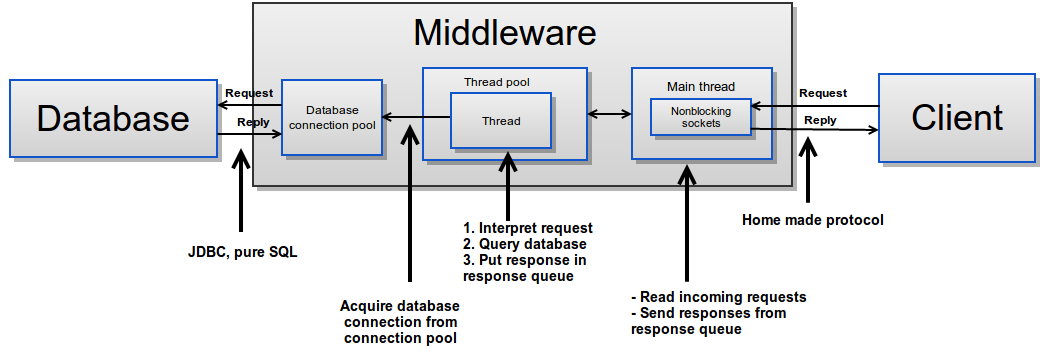
\includegraphics[scale=0.50]{implementation_high_level}
             \caption{Graphical representation of implementation}
             \label{fig:implementation_high_level}
         \end{figure}
         \begin{enumerate}
             \item Client sends SendMessage request to middleware
             \item Middleware receives request on non-blocking socket in the main thread
             \item Middleware passes raw request data on to thread X from the thread-pool
             \item Thread X interprets the request
             \item Thread X fetches a database connection from the database connection-pool, and performs a query
             \item Depending on the result of the query, thread X figures out what to respond to the client and puts the response in the response queue
             \item Next time the main thread looks through the response queue, it will pass on the response to the client
         \end{enumerate}

        \noindent In the following subsections we explain our design decisions with regard to each component of our system: client, middleware, and database.\\
        \\
        TODO: Describe API between server and client.


        \subsection{Client}
            We decided to keep the implementation of our client as simple as possible. This means that our client implementation only consists of code that implements the API described earlier. Basically, our client code is a library that can be used in other Java applications to communicate with our middleware.\\
            \\
            The client has the following important Java \textbf{packets} and \textit{classes}:
            \begin{itemize}
                \item \textbf{asl}
                    \begin{itemize}
                        \item \textit{ThorBangMQ} - Main class
                        \item \textit{Message} - Representation of a message
                    \end{itemize}
                \item \textbf{asl.network}
                \begin{itemize}
                     \item \textit{SocketTransport} - Transport layer using sockets
                 \end{itemize} 
                \item \textbf{asl.infrastructure}
                 \begin{itemize}
                    \item \textit{MemoryLogger} - Logging to memory, dump to file later
                \end{itemize}
                \item \textbf{asl.infrastructure.exceptions}
                \begin{itemize}
                    \item \textit{InvalidClientException} - Invalid client id
                    \item \textit{InvalidQueueException} - Invalid queue id
                    \item \textit{InvalidMessageException} - Invalid message id
                    \item \textit{ServerException} - Unknown exception at server, something is very wrong
                \end{itemize}
            \end{itemize}

        \subsection{Middleware}
            In our middleware we have chosen to use non-blocking sockets instead of blocking sockets since it as a few properties that we like, one of which is that we don't have to spawn a new thread for every client that connects. This means that it will have a smaller impact on the server when a client connects, and that we can support many more clients simultaneously, since the amount of threads in our program doesn't have to be linear to the amount of clients currently connected. There is an obvious disadvantage to choosing non-blocking sockets over blocking sockets though, which is that it can be harder to think about, implement, and work with non-blocking sockets.\\
            \\
            In an attempt to make our implementation simpler, we decided to perform all network i/o in one thread of our program. Since we want to be able to handle multiple requests simultaneously, we pass data from the network i/o-thread to worker threads for interpretation and handling. These worker threads interpret incoming data and perform database queries needed to complete the request. Afterwards they put the response in a response queue, which the network i/o-thread will read in order to send replies to the requesting clients.\\
            \\
            By moving interpretation and handling of requests to a thread different from the network i/o-thread, we have a place to perform our (blocking) queries to the database without blocking the whole system.\\
            We have chosen to use a thread-pool for request interpretation in order to avoid the overhead of creating and deleting threads all of the time, and at the same time bound the maximum number of threads our program will spawn. This should make our system able to handle many more clients than we have threads at the cost of slower response times.\\
            \\
            With regard to database connections, we have chosen to use a connection-pool to avoid the overhead of setting up a new connection to the database each time we query it.\\
            \\
            The middleware consists of the following important Java \textbf{packets} and \textit{classes}:
            \begin{itemize}
                \item \textbf{asl}
                \begin{itemize}
                    \item \textit{Main} - Entry point of the program
                    \item \textit{IntervalLogger} - Logs test data every x second, configurable
                    \item \textit{GlobalCounters} - Holds global counters used during tests
                    \item \textit{Message} - Representation of a message
                    \item \textit{ServerSettings} - Configurable parameters of the server
                \end{itemize}
                \item \textbf{asl.infrastructure}
                \begin{itemize}
                    \item \textit{MemoryLogger} - Logging to memory, dump to file later
                \end{itemize}
                \item \textbf{asl.infrastructure.exceptions}
                \begin{itemize}
                    \item \textit{InvalidClientException} - Invalid client id
                    \item \textit{InvalidQueueException} - Invalid queue id
                    \item \textit{InvalidMessageException} - Invalid message id
                    \item \textit{ServerException} - Unknown exception at server, something is very wrong
                \end{itemize}
                \item \textbf{asl.network}
                \begin{itemize}
                    \item \textit{SocketTransport} - Transport layer using sockets
                \end{itemize}
                \item \textbf{asl.persistence}
                \begin{itemize}
                    \item \textit{PostgresPersistence} - Uses Postgres as storage
                    \item \textit{InMemoryPersistence} - Uses local memory as storage
                    \item \textit{LyingPersistence} - Doesn't store anything
                \end{itemize}
            \end{itemize}

        \subsection{Database}
            We have chosen to use a simple database schema with three tables: messages, queues, and clients. We have put indexes on all fields that will be used to filter messages. These fields are indicated with a plus sign ($+$) on Figure \ref{fig:database_schema}. 
            \begin{figure}[H]
                \centering
                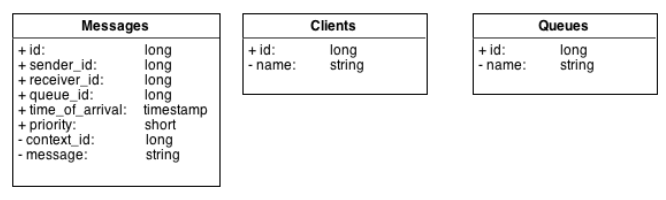
\includegraphics[scale=0.50]{database_schema}
                \caption{Database schema}
                \label{fig:database_schema}
            \end{figure}
            In order to allow clients to send messages to multiple queues at once, we have chosen to replicate messages in queues rather than having a many-to-many relationship in the database. This could obviously have an impact on performance.\\
            \\
            Communication between the middleware and our database is done using JDBC, making SQL queries directly from our Java code. We decided not to use stored procedures even though it requires slightly less data to represent each query, because we found it easier to implement and debug SQL directly in our Java code. 

        \subsection{Communication protocol}
            We have chosen to use a very simple messaging protocol between the clients and the middleware. We have chosen to use an end of message token to differentiate messages from each other, as we found it simpler to implement than defining packets with headers etc. We decided that our end of message token should be null, i.e. "\textbackslash\textbackslash0". All messages should be encoded in UTF8.\\
            Interpretation of messages is implemented in both server and client, in the DefaultTransport- and SocketTransport classes, respectively.

    \section{Testing infrastructure}
        Our testing infrastructure is written in Python and does the following:
        \begin{itemize}
            \item Starts and stops servers
            \item Starts and stops experiments
            \item Fetches logs
            \item Generates graphs
        \end{itemize}

    \section{Tests}
        In our tests we have focused on peeking, popping, and sending messages. We decided to have this focus because we assume that these requests are vastly more frequent than all other types of requests, e.g. create queue, and that the performance of these three types of requests will greatly dominate the performance of the other types.\\
        \\
        We have performed our tests using machines from the cloud hosting provider DigitalOcean.com, where we got a 200\$ coupon to run experiments. Running our tests on a cloud host has some obvious downsides w.r.t. our test results since we can't know for sure which hardware our tests are run on, and if we have any neighbors on this hardware.\\
        We have run all of our experiments on machines with: 4GB memory, SSD storage, and 2 logical CPU cores. Due to the way DigitalOcean provides their servers, we can't really tell how much computing power these logical CPUs provide, or whether there are any neighbors on the hardware. In order to compensate for this we've run all of our experiments for at least 10 minutes each, to check that the performance is somewhat consistent.
        \\
        To explain the performance of our system, we have identified the following parameters which we wish to test.
        \begin{itemize}
            \item Client
            \begin{itemize}
                \item Number of clients per server
                \item Total number of clients
                \item Type of test performed
            \end{itemize}
            \item Middleware
            \begin{itemize}
                \item Number of connections to database
                \item Number of worker threads
                \item Impact of using database vs. not storing messages at all
            \end{itemize}
            \item Database
            \begin{itemize}
                \item Indexes
            \end{itemize}
        \end{itemize}

        \subsection{Send message, pop message}
            We want to use this test to see how the amount of clients impacts the performance, as well as to see how the ratio between database connections and worker threads impacts the performance.\\
            In this test clients continuously send 'SendMessage' and 'PopMessage' requests to the server. It should be noted that the clients will block until receiving a response from a request, meaning that the throughput of both types of requests should be the same. Sending requests in this manner ensures that we keep the amount of messages in the database consistent.

        \subsection{Standard test}

        \subsection{Pure pop message}
        \subsection{Pure send message}
        \subsection{Pure peek message}

        \subsection{Mixed requests}
            \begin{itemize}
                \item Simulation of 'real workload'?
            \end{itemize}

        \subsection{Database connections vs. worker threads}
            This is a $2^2$ test.

        \subsection{Number of messages connections vs. time of reads}
            This is a $2^2$ test.

    \section{Results}
        TODO: Note that we're using a closed system which has an effect on the results\\
        TODO: Show raw data, graphs, do statistical treatment of data

        \subsection{Time spent in each part of the system}
            % Use test sendAndPopSameClient 2013-11-09__22_23_35 and 2013-11-09__22_24_23 to infer this.

        \subsection{Time to perform pop}

        \subsection{Time to perform peek}

        \subsection{Time to perform send}


    \section{Analysis}
        TODO: Interpret results showed above

    \section{Conclusion}
        TODO: Say something about performance of system\\
        TODO: Say something about what we could've done differently
    \section{Appendix}
        \subsection{Message protocol}
            \subsubsection{Exceptions}
                If a request cannot be fulfilled by the server, it will respond with an exception.  Exceptions have the following format:\\
                \\
                \indent\textit{FAIL $<$type$>$ $<$id$>$}\\
                \\
                Where $<$type$>$ is either QUEUE, CLIENT, MESSAGE, or UNKNOWN, and where $<$id$>$ is the id of the queue, client or message that ‘failed’. For instance, if a client tries to send a message to the queue with id 5 and if that queue doesn’t exist, the server will respond with “FAIL QUEUE 5”.

            \subsubsection{Handshake}
                The client should send HELLO when first connecting to the server. The server should respond with OK if it accepts the client, otherwise the server should respond with something else. The client must disconnect if it receives anything other than OK from the server.


            \subsubsection{Send Message}
                \indent\indent\textit{MSG,ReceiverId,SenderId,QueueId,Priority,Context,Content}\\
                \\
                \textbf{Response}\\
                The server should respond with OK if the message was inserted into the queue successfully, otherwise it should respond with FAIL.\\
                \\
                \textbf{Remarks}\\
                To send a message to multiple queues, separate the QueueIds with a semicolon, e.g. 1;2;3 to send the message to queues 1, 2 and 3.

            \subsubsection{Message Response}
                \indent\indent\textit{MSG,SenderId,Context,MessageId,Content}\\
                \\
                This is here to save space in the definitions below. This is how the server should return a message upon request from the client.

            \subsubsection{Peek Queue}
                \indent\indent \textit{PEEKQ,ReceiverId,QueueId,OrderByTimestampInsteadPriority}\\
                \\
                \textbf{Response}\\
                The server should respond with the message formatted as in section 1.2 if there is a message in the queue. Otherwise the response should be MSG0.\\
                \textbf{Remarks}\\
                OrderByTimestampInsteadPriority is either 1 or 0.

            \subsubsection{Peek Queue with Specific Sender}
                \indent\indent\textit{PEEKS,ReceiverId,QueueId,SenderId,OrderByTimestampInsteadPriority}\\
            \\
            \textbf{Response}\\
            The server should respond with the message formatted as in section 1.2 if there is a message in the queue. Otherwise the response should be MSG0.\\
            \\
            \textbf{Remarks}\\
            OrderByTimestampInsteadPriority is either 1 or 0.


            \subsubsection{Pop Queue}
                \indent\indent\textit{POPQ,ReceiverId,QueueId,OrderByTimestampInsteadPriority}\\
                \\
                \textbf{Response}\\
                The server should respond with the message formatted as in section 1.2 if there is a message in the queue. Otherwise the response should be MSG0.\\
                \\
                \textbf{Remarks}\\
                OrderByTimestampInsteadPriority is either 1 or 0.

            \subsubsection{Pop Queue with Specific Sender}
                \indent\indent\textit{POPS,ReceiverId,QueueId,SenderId,OrderByTimestampInsteadPriority}\\
                \\
                \textbf{Response}\\
                The server should respond with the message formatted as in section 1.2 if there is a message in the queue. Otherwise the response should be MSG0.\\
                \\
                \textbf{Remarks}\\
                OrderByTimestampInsteadPriority is either 1 or 0.

            \subsubsection{Create Queue}
                \indent\indent\textit{CREATEQUEUE,NameOfQueue}\\
                \\
                \textbf{Response}\\
                The server should respond with the id (long) of the queue, if a queue with the same name exists the server should respond with FAIL.

            \subsubsection{Remove Queue}
                \indent\indent\textit{REMOVEQUEUE,QueueId}\\
                \\
                \textbf{Response}\\
                The server should respond with OK or FAIL.

\end{document}
